\chapter{The South African and International Exhibition in Kimberley, 1892}

\ph[width = .90\textwidth]{../cape-of-good-hope/Exhibition/Kimberley-Exhibition.jpg}{
Official printed exhibition envelope  sent to Wellington ex 
Cape Town bearing triple oval violet cachet 
SOUTH  AFRICAN AND INTERNATIONAL EXHIBITION 
KIMBERLEY 1892, signed by Mrs J Alf Ellis  
exhibition secretary and dated 19.7.92, 
"compass wheel" dispatch cancel of Cape  Town. 
Circular letter included in envelope from the Local 
Committee Cape Town section  soliciting items 
suitable for exhibiting.}




 
\begin{marginfigure}
\centering
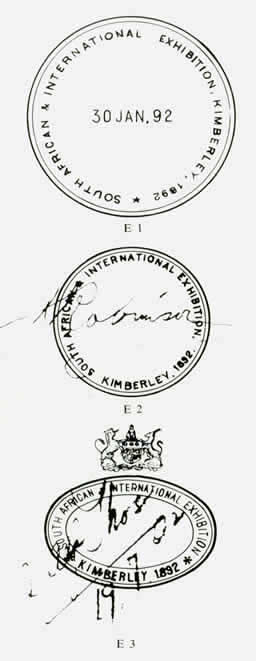
\includegraphics[width=0.95\textwidth]{../cape-of-good-hope/Exhibition/Exhibition-Postmarks.jpg}
\end{marginfigure}

 

The South African and Internatonal Exhibition was staged in Kimberley 
in 1892. It was opened by Sir Henry Loch, the then Governor of 
the Cape of Good Hope on the 8th of September. It presented 
exhibits of art, an exhibition of paintings from the royal 
collection of Queen Victoria and mining machinery and implements 
amongst other items. The exhibition aroused considerable interest 
at internationallevel, which resulted in a competition for display space.
Kimberley Exhibition Postmarks

The government of the Cape of Good Hope allowed the secretary of the
exhibition free franking privileges, before the opening of the event. 
Three exhibition cachets are known (E 1,E 2 and E 3).
Exhibition Postmarks E-1
 

The earliest exhibition covers E1 has a double circle design and 
has a diameter of 53 mm. It reads "South African and International 
Exhibition, Kimberley, 1892". There is a star at the bottom and the 
date is located centrally.

The second in the series (E 2) also has a doubled lined circle design. 
The diameter is 40 mm.The wording is the same as E 1, 
but there is no star. It has the signatue of Mr. Robinson the 
secretary to the exhibition.

E 3 is a tremble-lined oval surmounted by a crest of the arms 
of the Cape of Good Hope. The endorsement of J. Al Ellis, 
secretary of the Cape Town committee of the exhibition. The only known 
cover is dated 19.7.1892. This cover which is illustrated 
above had a letter enclosed canvassing contributions from the 
Cape of Good Hope socialites.

Another postmark E 4, indicates that a temporary post office 
was opened at the exhibition, and that the Cape of Good Hope 
authorities provided a special date stamp for the occassion. 
(The exhibition brochure mentions that the postal facilities 
would be available to exhibitors and visitors).

However, a poscard in my possesion though shows correspondence 
emanating from the exhibition franked with the single circle 
Cape Town mark does not show such a mark. This post card is illustrated below.

\ph[width = .50\textwidth]{../cape-of-good-hope/Exhibition/card.jpg}{ }

\ph[width = .95\textwidth]{../cape-of-good-hope/Exhibition/Kimberley-exhibition-front.jpg}{ }

The scarcity of this postmark is somehow difficult to explain as in the 
\textit{Philatelic Record}\sidenote{Vol. XIII. NOVEMBER, 1891. No. 155, p.276} the following notice
appeared:

\begin{blockquote}
Mr. C.N.Biggs informs us that he has had a communication from
Captain Charles Morris-Newman, of Aliwal North, Cape Colony, South Africa, in which the following information is given: "We have
started a small Philatelical Society here in South Africa, with its head
quarters at Port Elizabeth, and as they intend having an exhibition next
year at Kimberley, we are endeavouring to have a section set apart for philately, when I shall make an effort and try and show my collection
of nearly 10,000, which I have got together in thirty years' wanderings."
Philately is evidently" on the boom " in Africa! We wish every
success to Captain Newman in his ventures, and shall be pleased to give him all the aid that lies in our power through the columns of the
Record.
\end{blockquote}

Any envelope around this date and addressed to a Charles Morris-Newman should be examined very carefully!













 

                           